\documentclass{article}
\usepackage[utf8]{inputenc}
\usepackage[margin=1in]{geometry}
\usepackage[T1]{fontenc}
\usepackage{graphicx}
\usepackage{enumitem}
\usepackage{pdfpages}

\begin{document}

\begin{titlepage} % Suppresses displaying the page number on the title page and the subsequent page counts as page 1
	\newcommand{\HRule}{\rule{\linewidth}{0.5mm}} % Defines a new command for horizontal lines, change thickness here
	
	\center % Centre everything on the page
	
	%------------------------------------------------
	%	Headings
	%------------------------------------------------
	
	\textsc{\LARGE University of Manitoba}\\[1.5cm] % Main heading such as the name of your university/college
	
	\begin{figure}
	    \centering
	    
\includegraphics[width=1in]{uofmlogo.png}
	    \label{fig:uofm}
	\end{figure}
	
	\textsc{\Large COMP 3020}\\[0.5cm] % Major heading such as course name
	
	\textsc{\large Human Computer Interaction I}\\[0.5cm] % Minor heading such as course title
	
	%------------------------------------------------
	%	Title
	%------------------------------------------------
	
	\HRule\\[0.4cm]
	
	{\huge\bfseries Group 20: Milestone 4}\\[0.4cm] % Title of your document
	
	\HRule\\[1.5cm]
	
	%------------------------------------------------
	%	Author(s)
	%------------------------------------------------
	
	\begin{minipage}{0.4\textwidth}
		\begin{flushleft}
			\large
			\textit{Authors}\\
			Skylar \textsc{Greenslade}, 7795032\\
			Sanjay \textsc{Abraham}, 7793952\\
			Seunghwan \textsc{Youn}, 7846681
			
		\end{flushleft}
	\end{minipage}
	~
	\begin{minipage}{0.4\textwidth}
		\begin{flushright}
			\large
			\textit{Professor}\\
			Dr. Jim \textsc{Young} % Supervisor's name
		\end{flushright}
	\end{minipage}

	
	\vfill\vfill\vfill % Position the date 3/4 down the remaining page
	
	{\large\today} % Date, change the \today to a set date if you want to be precise

	\vfill % Push the date up 1/4 of the remaining page
	
\end{titlepage}
\newpage

\section{Heuristic Evaluation Method}
%describe method, individually, and group.

After creating the high-fidelity prototype for Milestone 3, our group began the evaluation process. First, each of our three group members individually performed a heuristic analysis, then one more heuristic analysis was performed as a group. Each individual evaluation took approximately one hour, and detailed notes were taken throughout the process. The interface was examined thoroughly from the first screen seen when it was started, through the process of planning and changing schedules, and all minute details of each aspect of the interface were considered. The evaluation was based on Jakob Nielson's ten heuristics. The evaluators considered each item in the list of heuristics when examining each element of the interface, and recorded any shortcomings regarding that item.
\newline
\newline \noindent
Once all group members had performed their individual analyses, the team met for the group heuristic analysis. This process was very similar to the individual analyses, in that the same heuristics were considered, and a very similar approach was taken to ensure each element of the design was covered. Each group member contributed their findings, and any other observations made for each section of the design, and notes were taken in a group document. The group also discussed what elements had the strongest negative impact, and were most important to be addressed. If more work is do be done on the design, a decision matrix could be created to include the expected time to make the changes, but for the sake of this milestone, only the severity of the heuristic violations were considered.

\section{Identified Issues}
%describe issues identified, along with which heuristics were violated, and finally, how you would address them in another iteration

The problems and heuristic violations are recorded here for each conceptual area of the design. The items in each area are ordered by their significance, and potential solutions discussed for each. The related heuristic is also listed as a reference, and the violation is elaborated on in the description.

\subsection{Information Card}

\subsubsection{Aesthetic and Minimalist Design}
The information provided in the help card can be improved. Although it is useful, it is not necessarily concise, and the aesthetic does not encourage being read. This card should be reworked in a future iteration to include only pertinent information, and in a format that is simple to understand.

\subsubsection{Help and Documentation}
Even though there is enough information in the card for a user to be able to use the interface, there are some important features that are not explained in the description. More direct instructions such as "search for classes here" near the search bar, and "add classes by clicking here" by the "add classes" button would be useful information, while still being quickly understood. Ideally, instruction is not required for all users, but the documentation should be able to answer any questions about how to user the interface.

\subsubsection{Recognition Rather Than Recall}
The correlation between the minimize button on the information card, and the information icon in the priority list could be stronger. Currently there is no indication that the information icon will lead to the information card, unless it is assumed that it is the only information that the user will receive. A short animation that shows the information card shrinking into the information icon would help to solidify the relationship between the two, and help the user to recognize the connection. Adding mouse over text on the information icon would further affirm its function, and prevent the user from having to guess at its use.


\subsection{Search Bar}


\subsubsection{Help Users Recognize, Diagnose, Recover From Errors}
Currently, when a user attempts to add a class to the planner that is already there, it does not let them, and the only feedback they receive is the search bar outline becoming red. Some kind of message should tell the user that they cannot add a class because it is already in the planner so that they are not left confused or frustrated.

\begin{figure}[h!]
    \centering
    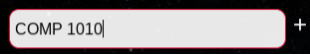
\includegraphics[width = 0.6\textwidth]{AddClassesError.png}
    
    \caption{A red border is the only feedback given when a course cannot be added}
    \label{fig:addClassError}
\end{figure}


\subsubsection{Error Prevention}
The course search bar will suggest any courses that match the given input, including those that are already added to the planner. This can lead to errors, as the system does not allow adding a class twice. By simply not suggesting courses that cannot be added, needless errors can be prevented.


\begin{figure}[h!]
    \centering
    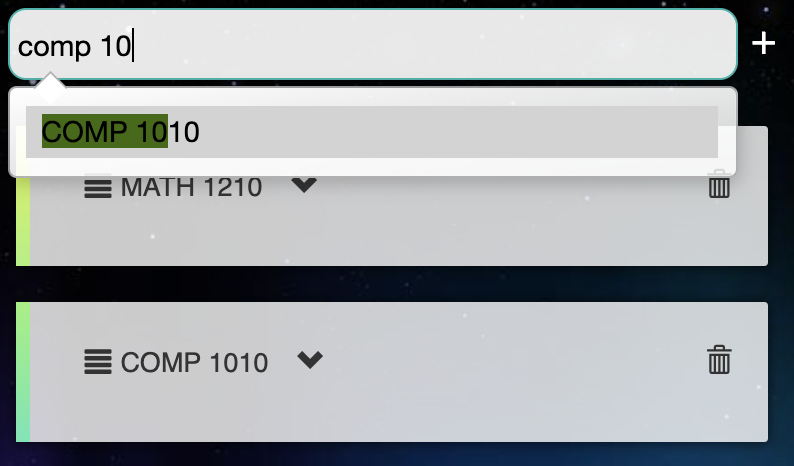
\includegraphics[width=0.6\textwidth,]{duplicateCourse.png}

    \caption{Search bar suggests a courses which was already added to the planner}
    \label{fig:duplicateCourse}
\end{figure}


\subsubsection{Recognition Rather Than Recall}
The add course button ('+' button as seen in Figures \ref{fig:addClassError} and \ref{fig:duplicateCourse}) on the interface is currently rather small and thin. This makes it hard to see, and a user may have difficulty noticing it initially. To help to user recognize the functionality sooner and throughout their use of the design, the icon should be larger, and thicker.


\subsubsection{Match Between System and Real World}
When using the search bar to find a class, the search bar only accepted and suggested course codes (ie: COMP 3020). It is possible that some users might not know the course codes for all of the classes they may want to take. Users may refer to classes by their names, so to match the system to the real world better, the user should be able to search for classes by their names, in part or in whole. The suggestions should also indicate the course name in some way, especially if the user is searching using a title instead of a course code.


\subsubsection{Flexibility and Efficiency of Use}
Although a user can add courses using only the keyboard, and no mouse actions, if the mouse is also used, it takes two separate mouse clicks. One to select the course from the suggestions, then one more to add it to the planner. If the user clicks on a course to add it, there is no need to require a second input. Clicking on the desired course should add it immediately, improving the efficiency of the interface.



\subsection{Priority List}

\subsubsection{Consistency and Standards}
The course cards in priority list appear as though they should be interactive from anywhere on the card, but that is not the case. Clicking on the card expands the card to show the individual sections within it, as well as some basic information. The prototype currently allows the user to click on the card anywhere in the center section, but not close to the edges of the card. Dragging the cards to reorder them is even more limited, as it only works on the drag icon. Both of these functions should be accessible from clicking anywhere on the card, as is typical with similar interface elements.

\begin{figure}[h!]
    \centering
    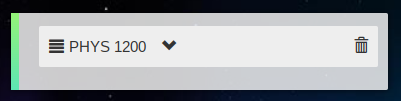
\includegraphics[width = 0.6\textwidth]{dragndrop}
    \caption{Highlighted area on a course card showing where to click to expand it}
    \label{fig:dragndrop}
\end{figure}


\subsubsection{Visibility of System Status}
The main course cards have a downward facing arrow (as seen in Figure \ref{fig:dragndrop}) to indicate they can be expanded, which inverts when expanded to indicate that the card can be collapsed. The individual sections within the course card have a similar functionality, however, they do not have any icon to indicate this. Including the arrow would make a more consistent interface, but more importantly, it would inform the user of the functionality present.




\subsubsection{Help Users Recognize, Diagnose, Recover From Errors}
When a class cannot be fit into a schedule, it is given a bright red border to indicate this. Although it should be immediately apparent to a user what classes are included in a schedule, and which are not, it is not as clear why a class is not included, and what the user needs to do to include it. Adding some kind of message to tell the user these pieces of information would greatly help the user know what to do next if they do not actually have their list in their preferred order. Simply telling a user that a class does not fit is not very helpful in that regard.



\subsubsection{Help Users Recognize, Diagnose, Recover From Errors}
When a user deletes a class, they can re-add it by using the search bar again, and dragging it to its original position in the priority list. This is many more steps than should be necessary to undo an action, so an undo function should be included in the design. This can be accomplished using standard shortcuts ("ctrl" + "z"), or by adding an undo button after a course is deleted. This way, any mistakes can be undone quickly, and without causing the user any stress.


\subsubsection{Visibility of System Status}
When the priority list becomes longer than can fit on one screen, a scroll bar is introduced. The scroll bar is quite thin, and it is hard to tell which part of it is the scroll bar, and which part is the background plate for the scroll bar. This can lead to confusion about what part of the list is being viewed, and which way to scroll to see the rest of it. To fix this violation, changing the colour or size of the scroll bar could help, as well as eliminating the background plate for it.

\subsubsection{Consistency and Standards}
The individual course sections that are deselected are greyed out and clearly indicate that they will not be included in the schedules. When a course is in the list but not included in any schedule, it would be more apparent to the user if it also greyed out. This would create consistency in the interface.

\begin{figure}[h!]
    \centering
    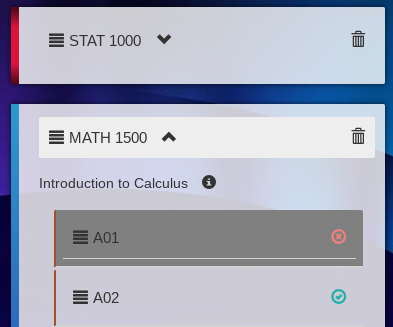
\includegraphics[width=0.6\textwidth]{deselectedSection.png}

    \caption{An unscheduled course remains light grey, while a deselected course section is greyed out}
    \label{fig:deselectedCard}
\end{figure}



\subsubsection{Help and Documentation}
The user is able to disable specific sections of a course if they so choose. This allows more control over the planner, however this functionality is not explained anywhere in the interface. Some documentation should be available to describe this function, so that it does not rely on the user's exploration and experimentation to discover it.



\subsubsection{Recognition Rather Than Recall}
The colours of the cards on the priority list as well as the blocks on the schedule are designed to be useful, both to indicate priority, and to show what pieces of information are related across the interface. To ensure that this is the case for all users, colours or designs should be chosen so that users with colour blindness.



\subsubsection{Visibility of System Status}
The algorithm which creates the schedules does not always include every section of a class if they do not fit. This is expected, however there is no indication to the user of what sections are and are not included in any possible schedule aside from manually viewing each one. A similar system could be implemented to the courses where included classes are given a border of the related colour, and unincluded classes are indicated as such with red. 



\subsubsection{Consistency and Standards}
Individual course sections in the course cards expand and collapse smoothly when clicked. The course cards themselves have a similar expand and collapse function, but they do so instantly, without any smooth animation. To keep the interface consistent, the source cards should also have this animation effect.


\subsubsection{Consistency and Standards}
The drag icon on the course cards is the same icon as is used to represent the "justify" text option for word processors. This icon should be switched to a standard drag icon instead.

\begin{figure}[h!]
    \centering
    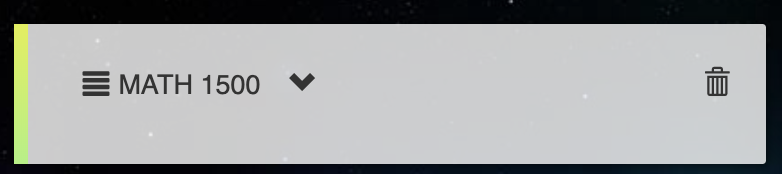
\includegraphics[width=0.6\textwidth]{dragicon.png}
    \caption{The "justify" icon being used in place of a standard "drag" icon}
    \label{fig:dragicon}
\end{figure}




\subsubsection{Flexibility and Efficiency of Use}
When many individual course sections are expanded within a course card, it can become quite large, especially if there are many sections available. This may prevent being able to see other course information as the user would like. When the course card is collapsed, it becomes a small, unobtrusive size again, but on expansion, it retains all of the expanded course sections from before. When the course card is collapsed, all individual course sections should also be collapsed, so that the card does not become unexpectedly, and obtrusively large when expanded again.




\subsubsection{Visibility of System Status}
The course cards are colour coded to match the blocks in the schedules presented. They are also colour coded to indicate priority, high priority being a brighter colour, and lower priority being more muted. The lowest priority colour is a deep purple, which blends into the background and is not always easy to see. Changing this colour to be higher contrast, and adding more shadow to the course cards would mitigate this issue and increase the visibility of the system status.


\subsubsection{Visibility of System Status}
When the course cards are expanded to show the individual sections and the information for each individual section, they can become quite long. They still have the colour coded border on the side, and the gradient becomes more gradual. This introduces a problem with the third and fourth priority cards, where the colours appear very similar when their cards are expanded enough. This may cause confusion as to which blocks on the schedule they are referring to. To make their status more clear, more contrast between the bottom colour of the third item and the top colour of the fourth item should be used.


\subsubsection{Visibility of System Status}
The prototype instantly updates the user's schedules once they modify their priority list. This is important functionally, but it does not really show what is happening when changes are made. If a stronger connection is made between the interactions in the sidebar and the output of the schedules, it may improve the user's understanding of system status and how the priority system works.



\subsection{Schedule Display}

\subsubsection{Help Users Recognize, Diagnose, Recover From Errors}
Our research indicated that one of the most important factors for users is the times that they will be at the university. The way that the schedule window is displayed does not make it very clear what time each block may start at. Adding minor vertical lines and adjusting the time heading to be more precise would help the users be able to create their ideal schedule faster, and without mistakes.


\begin{figure}[h!]
    \centering
    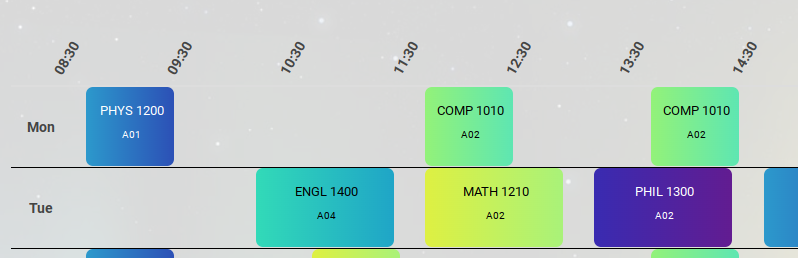
\includegraphics[width = 0.9\textwidth]{sched2.png}
    \caption{Schedule Display showing 24 hour format times}
    \label{fig:sched}
\end{figure}



\subsubsection{Flexibility and Efficiency of Use}
To access more detailed information about a course, the course card must be expanded and the relevant button there clicked on. When the user is focused on the schedules presented to them, they may want to view this information without having to disrupt their mental process and navigate through the other part of the interface. The user should be able to access this information by clicking on a block on the schedule, or an information button on a course's block. This would make the usage of this system more flexible and more efficient.



\subsubsection{Consistency and Standards}
The schedule shows the times in a 24 hour format, whereas the course cards list the time in a 12 hour format. To remain consistent across the interface, these two formats should be the same.


\subsubsection{Flexibility and Efficiency of Use}
When a user decided that they want to include a specific section of a course no matter what, they can do so by deselecting all other sections of that course, and dragging that course to the top of the priority list. This takes quite a few steps, and is a bit for a workaround to a feature that many users may appreciate. If the user is given the ability to "lock" a section in like this by clicking on it in the schedule, this could greatly improve the efficiency of the system, as well as allowing users to plan in more ways that might seem more natural to them.


%this one's (below) kinda weak? vvv
\subsubsection{Match Between System and Real world}
When the user scrolls through the various schedule options presented to them, they instantly appear. A fast animation which showed the schedules appearing and disappearing could indicate better to the user what is happening, and relate the abstract nature of a schedule more to the tactile world.




\subsection{More Information Section}




\subsubsection{Consistency and Standards}
To bring up the detailed information for a course, the button is another information "i". This makes sense, but a similar version of the same icon was used to bring up the help card. Using a very similar button for different functions may be confusing to the user, so a distinct button should be used instead. 

\begin{figure}[h!]
    \centering
    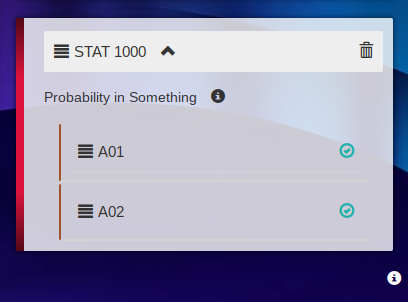
\includegraphics[width=0.55\textwidth]{moreInfo.png}

    \caption{The "more information" button on the course card matches the "Information Card" button}
    \label{fig:moreInfo}
\end{figure}


\subsubsection{Recognition Rather Than Recall}
The "i" button is typically used for extra information that is not necessary for all users. In this prototype, it was used for a very important feature, and is not described elsewhere. Using a more appropriate icon would help to address this violation, as well as having some mouse over text or similar to inform the user.

\subsubsection{Aesthetic and Minimalist Design}
The More Information section has a darker background compared to the rest of the interface. This perhaps does not match the aesthetic of the rest of the design. It also might portray a different mood than intended. A bit more colour or a lighter background may help to produce a more cohesive interface, and be more enjoyable for users.



\section{Conclusion}
%review most important findings and recommendations
By performing multiple heuristic analyses of the prototype, many issues were identified. A lot of issues could be addressed with better feedback and documentation. Some simple yet important changes would greatly improve the consistency within the interface, as well as improving the visibility of the system's capabilities. Examples of this are changing icons to standards, matching time formats, and greying out cards appropriately. Some changes such as reworking the documentation would take more work and research to implement well, but can still be fixed without overhauling the main design. 
\newline  
\newline \noindent 
Although the significance of the heuristic violations do vary, all of them could be addressed, and likely with a relatively small amount of work. A second iteration of this prototype would be able to incorporate solutions to all of the issues as mentioned in this report, and further evaluation and testing could be performed. Overall this evaluation yielded good results in finding how the design can be improved and made to be a successful interface.








\newpage	
\pagenumbering{gobble}
\vspace*{40mm}
\begin{centering}
	{\huge\bfseries Appendix G: Raw Individual Heuristic Evaluation Notes}\\[0.4cm] 
\end{centering}





\newpage	
\pagenumbering{gobble}
\vspace*{40mm}
\begin{centering}
	{\huge\bfseries Appendix H: Group Heuristic Evaluation Notes}\\[0.4cm] 
\end{centering}





\end{document}